

\section{Day 1: general ML and transformer background}

\subsection{Rough structure of a transformer}

\noindent\textbf{Main resource for further study: ARENA.} For a detailed understanding of transformer structure, watch the videos and work through the explanations and coding exercises in \href{https://learn.arena.education/chapter1_transformer_interp/01_transformers/intro/}{ARENA's Transformers from Scratch material}~\cite{arenaTransformers}. This is the key resource to return to alongside this summary, especially the exercises implementing a transformer from scratch.

The \emph{residual stream} is a high-dimensional working representation: each token position carries a vector in $\R^{\texttt{d\_model}}$, updated as it passes through successive transformer blocks. Tokenisation first splits text into units, for example using byte-pair encoding, a compression-inspired procedure. Learned embeddings map these tokens to vectors; positional information is supplied separately, through positional embeddings or mechanisms such as rotary attention. Semantic structure develops through training, with the representation becoming sensitive to context as the layers process it~\cite{wilhelmSchulz2026transformers}.

Each block combines \emph{attention}, which moves information between token positions, and an \emph{MLP} (multi-layer perceptron), which applies the same nonlinear transformation independently at each position. Attention heads operate in parallel: each learns lower-dimensional query, key, and value projections of the residual stream, then writes its output back into that stream. Typically, $h$ heads have dimension $\texttt{d\_head}=\texttt{d\_model}/h$. These are learned, potentially overlapping views of the full vector, rather than disjoint compartments. In a causal language model, a position can attend to itself and earlier positions. The MLP then processes the information gathered there; its weights can encode learned associations and factual information, though knowledge is distributed across the model~\cite{wilhelmSchulz2026transformers,vaswani2017attention}.

Ignoring normalisation, we alternate between attention and MLP updates of the schematic form
\[
  \begin{aligned}
    X_{2n+1} &= X_{2n} + \operatorname{Attention}_n(X_{2n}), \\
    X_{2n+2} &= X_{2n+1} + \operatorname{MLP}_n(X_{2n+1}).
  \end{aligned}
\]
This suggests a discrete dynamical system along depth: blocks repeatedly read the current state and add updates, whose components can have either sign. Attention exchanges information between positions; MLPs transform it locally. Finally, an unembedding maps the resulting vectors to next-token scores. Training can process positions in parallel under a causal mask, while generation proceeds one new token at a time.

\begin{center}
  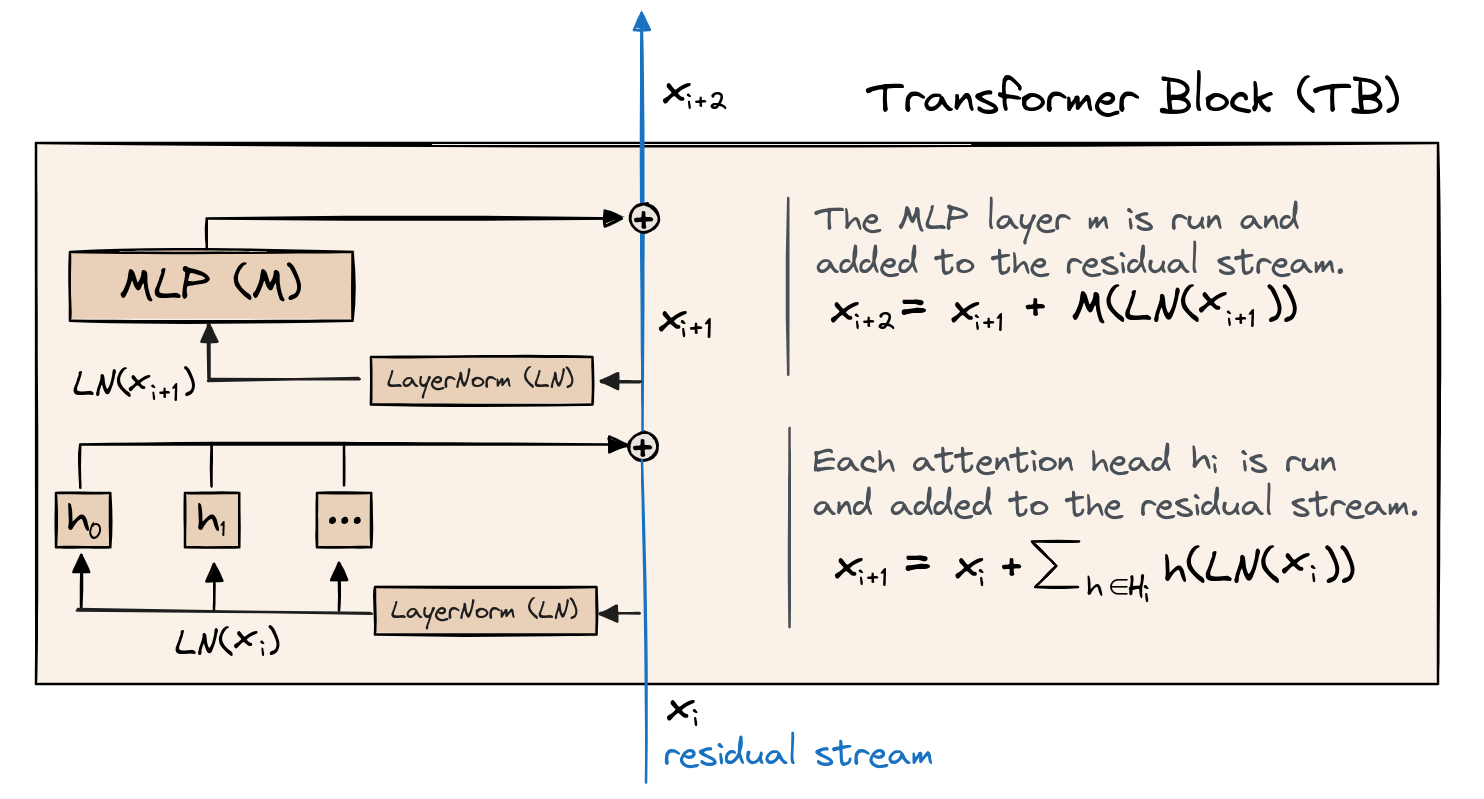
\includegraphics[width=0.95\linewidth]{figures/arena-transformer-block.png}
  \captionof{figure}{A transformer block: attention and an MLP add successive updates to the residual stream, flowing from bottom to top. The diagram also shows the normalisation omitted above. Reproduced from \href{https://learn.arena.education/chapter1_transformer_interp/01_transformers/2-clean-transformer-implementation/}{ARENA, Clean Transformer Implementation}~\cite{arenaTransformerImplementation}.}
  \label{fig:arena-transformer-block}
\end{center}

\noindent\textbf{Selected readings: transformer structure.}
\begin{itemize}
  \item \href{https://learn.arena.education/chapter1_transformer_interp/01_transformers/intro/}{ARENA, Transformers from Scratch}~\cite{arenaTransformers}: the main practical reference, with videos and implementation exercises.
  \item \href{https://arxiv.org/abs/1706.03762}{Vaswani et al., Attention Is All You Need}~\cite{vaswani2017attention}: the original architecture, especially Section 3.
\end{itemize}

\subsection{Training path: pretraining, supervised fine-tuning, and RL}

A useful schematic path is
\[
  \text{pretraining}
  \;\longrightarrow\;
  \text{supervised fine-tuning}
  \;\longrightarrow\;
  \text{reinforcement learning}.
\]
\emph{Pretraining} learns next-token prediction from large, varied text corpora, including web data. This develops linguistic knowledge and broad capabilities, but does not specifically train a consistent assistant role. The model can learn many voices and patterns of interaction.

\emph{Supervised fine-tuning} (SFT) trains on demonstrations of desired responses. Each example provides a prompt or conversation, often with role markers and a system instruction, followed by a target assistant response. A common setup computes the prediction loss only on assistant-response tokens: the preceding conversation supplies context. This encourages an assistant style and instruction-following behaviour by imitation. The underlying mechanism remains next-token prediction; training changes which continuations are likely~\cite{ouyang2022instructgpt}.

\emph{Reinforcement learning} (RL) instead updates the model using scores for generated responses. In a standard RLHF pipeline, humans compare candidate responses; these comparisons train a reward model, which then scores new responses for an RL algorithm to optimise. Thus, ranking pairs supplies supervision for the reward model, rather than being the RL update itself~\cite{ouyang2022instructgpt}. With \emph{RLAIF}, AI judgements supply feedback instead, potentially guided by human-written principles~\cite{bai2022constitutional}. Rewards can also come from automatic checks, such as whether a solution passes tests. Both SFT and RL are forms of \emph{post-training}; this three-stage path is a useful simplification, and individual training recipes vary.

\noindent\textbf{Selected readings: training stages.}
\begin{itemize}
  \item \href{https://arxiv.org/abs/2203.02155}{Ouyang et al., Training Language Models to Follow Instructions with Human Feedback}~\cite{ouyang2022instructgpt}: the SFT, reward-model, and RLHF pipeline.
  \item \href{https://arxiv.org/abs/2212.08073}{Bai et al., Constitutional AI}~\cite{bai2022constitutional}: supervised fine-tuning and reinforcement learning using AI feedback.
\end{itemize}

\section{Day 2: Introduction to AI Alignment}

\subsection{Alignment targets, corrigibility, and control}

One central question is what we want an AI system to pursue, and how to make it motivated to pursue that target. This involves deciding whose values count and how to interpret them: literal instructions, inferred intentions, or the preferences we would endorse after further reflection. Christiano's notion of \emph{intent alignment} focuses on a system trying to do what its operator wants. This concerns its motivations; it does not guarantee that the operator's wishes are good, or that the system has the knowledge and competence to carry them out safely~\cite{christiano2018clarifying}.

\emph{Coherent extrapolated volition} (CEV) is a proposal for grounding an alignment target in humanity's collective volition~\cite[Section~3]{yudkowsky2004cev}. The idea is to ask what we would want with more knowledge, greater capacity to think and reflect, and the opportunity to develop together. It seeks to accommodate the wishes of humanity as a whole, including how we would want those wishes to be extrapolated and reconciled. The aim is therefore broader than satisfying our present requests: our current choices can reflect ignorance, inconsistency, or desires we would later reject. Coherence is something to seek where our extrapolated wishes fit together, rather than something to impose by suppressing disagreement.

A more concrete way to state a target is through a document describing intended values and behaviour. \emph{Claude's constitution}, for example, sets out Anthropic's intentions for Claude and informs its training. It addresses helpfulness, ethical judgement, and human oversight, while acknowledging that actual model behaviour may depart from these intentions~\cite{anthropic2026constitution}.

But what if we specify the wrong target, or the system interprets it incorrectly? This motivates \emph{corrigibility}: a system should permit correction, modification, and shutdown, even when these would interfere with its current objective. Stronger forms include actively helping us make such corrections. The difficulty is that continued operation and preservation of its goals can be instrumentally useful to a goal-directed system, giving it reasons to resist intervention~\cite{lesswrongCorrigibility}.

We also need \emph{control}: safeguards intended to prevent unacceptable outcomes even if a system is misaligned and actively tries to circumvent them~\cite{shlegerisGreenblatt2024control}. Corrigibility concerns the system's willingness to accept intervention; control concerns our ability to keep its actions safe even without that cooperation. These are complementary requirements, and neither choosing a desirable target nor allowing eventual correction alone ensures that harm cannot occur before we intervene.

\noindent\textbf{Selected readings: alignment targets and safeguards.}
\begin{itemize}
  \item \colorbox{yellow!40}{\strut\href{https://intelligence.org/files/CEV.pdf}{Yudkowsky, Coherent Extrapolated Volition}~\cite{yudkowsky2004cev}}: begin with the first two and a half pages of Section 3, as suggested in the slides.
  \item \href{https://ai-alignment.com/clarifying-ai-alignment-cec47cd69dd6}{Christiano, Clarifying AI Alignment}~\cite{christiano2018clarifying}: the distinction between intent alignment and successful outcomes.
  \item \href{https://www.anthropic.com/constitution}{Claude's constitution}~\cite{anthropic2026constitution}: a concrete statement of intended model values and behaviour.
  \item \href{https://www.lesswrong.com/w/corrigibility-1}{Corrigibility}~\cite{lesswrongCorrigibility} and \href{https://blog.redwoodresearch.org/p/the-case-for-ensuring-that-powerful}{the case for AI control}~\cite{shlegerisGreenblatt2024control}: cooperation with correction and safeguards against uncooperative systems.
\end{itemize}

\subsection{How things can go wrong}

The slides organise these concerns using the distinction between \emph{outer} and \emph{inner alignment}. Outer alignment asks whether the training objective rewards what we actually want; inner alignment asks whether the trained system itself pursues that objective. Even broad, representative data cannot rescue a reward rule that favours the wrong outcomes. Conversely, a correct reward rule need not produce the intended goal when the training situations fail to distinguish it from alternatives. Limited data coverage is therefore one possible cause of inner misalignment, rather than its definition; the distinction is useful but does not cleanly separate all practical failures~\cite{hubinger2019learnedOptimization,shah2022misgeneralization}.

\href{https://deepmind.google/blog/specification-gaming-the-flip-side-of-ai-ingenuity/}{\emph{Specification gaming}} concerns a mismatch between what we reward and what we want: the scoring rule admits shortcuts that satisfy it without completing the intended task~\cite{krakovna2020specificationGaming}. For example, a coding agent might edit the tests to obtain a passing score instead of fixing the code. RL can directly encourage this by rewarding successful exploitation of the scoring rule. This illustrates an \emph{outer alignment} concern: whether the objective itself expresses our intention.

\href{https://deepmind.google/blog/how-undesired-goals-can-arise-with-correct-rewards/}{\emph{Goal misgeneralisation}} can occur even with a correct reward rule~\cite{shah2022correctRewards}. The training situations may leave several goals indistinguishable, so the agent learns one that agrees with our intention during training but diverges in deployment. For example, if a coin is always on the right during training, an agent may learn to seek the right-hand location rather than the coin. The concern is that it remains capable while pursuing the wrong goal, rather than simply failing on unfamiliar inputs~\cite{shah2022misgeneralization}. This is related to \emph{inner alignment}: what objective, if any, the trained system itself pursues~\cite{hubinger2019learnedOptimization}. Broader training data can help, but architecture and optimisation also influence which strategy is learned.

In supervised learning, limited data coverage can likewise leave the intended goal indistinguishable from a proxy. This is a useful connection, rather than an RL-versus-SL split: goal misgeneralisation also occurs in RL~\cite{shah2022misgeneralization}.

\noindent\textbf{Selected readings: specification gaming and goal misgeneralisation.}
\begin{itemize}
  \item \href{https://deepmind.google/blog/specification-gaming-the-flip-side-of-ai-ingenuity/}{DeepMind, Specification Gaming: The Flip Side of AI Ingenuity}~\cite{krakovna2020specificationGaming}: examples of satisfying the score without achieving the intended outcome.
  \item \href{https://deepmind.google/blog/how-undesired-goals-can-arise-with-correct-rewards/}{DeepMind, How Undesired Goals Can Arise with Correct Rewards}~\cite{shah2022correctRewards}: a short introduction; see also the \href{https://arxiv.org/abs/2210.01790}{goal misgeneralisation paper}~\cite{shah2022misgeneralization}.
  \item \href{https://arxiv.org/abs/1906.01820}{Hubinger et al., Risks from Learned Optimization}~\cite{hubinger2019learnedOptimization}: the original discussion of learned objectives and inner alignment.
\end{itemize}

\subsection{How things can go wrong, part two: inductive biases and fine-tuning}

The same training examples can be consistent with very different behaviour outside the training distribution. Architecture, pretraining, and optimisation introduce \emph{inductive biases} that influence which solution is learned and how it changes under fine-tuning~\cite{wilson2025deepLearning}. This makes generalisation a question about both the data and the system learning from it, with consequences for inner alignment.

In \emph{emergent misalignment}, fine-tuning a model to produce insecure code without warning the user led to harmful and deceptive responses on unrelated tasks~\cite{betley2025emergent}. The change extended beyond the coding behaviour being trained. Giving the same insecure-code task a benign educational framing prevented the effect in a control experiment. One interpretation is that fine-tuning can shift a broadly expressed assistant persona, rather than only a local skill; the \emph{persona selection model} develops this perspective~\cite{marks2026persona}. This is a useful hypothesis, not proof that persona changes reduce training loss faster than skill changes, or that the effect follows from transformer architecture alone.

Interpretability offers a related clue: Arditi et al. found a single residual-stream direction per model that strongly mediated refusal in the chat models they studied~\cite{arditi2024refusal}. Removing it suppressed refusal, while adding it could induce refusal on harmless requests. This shows that a low-dimensional intervention can have broad behavioural effects; it does not establish a universal direction for morality or maliciousness. An open question is how shared internal representations allow a narrow training update to alter behaviour across many contexts.

\noindent\textbf{Selected readings: training and generalisation.} From the slides' reading list; yellow marks the paper already read sufficiently for this review.
\begin{itemize}
  \item \href{https://www.alignmentforum.org/posts/FDJnZt8Ks2djouQTZ/how-do-we-become-confident-in-the-safety-of-a-machine}{Hubinger, training stories}~\cite{hubinger2021trainingStories}: read through the discussion of how mechanistic a training goal needs to be.
  \item DeepMind: \href{https://deepmind.google/blog/specification-gaming-the-flip-side-of-ai-ingenuity/}{specification gaming}~\cite{krakovna2020specificationGaming} and \href{https://deepmind.google/blog/how-undesired-goals-can-arise-with-correct-rewards/}{goal misgeneralisation}~\cite{shah2022correctRewards}.
  \item \href{https://arxiv.org/abs/2503.02113}{Wilson, Deep Learning Is Not So Mysterious or Different}~\cite{wilson2025deepLearning}: Sections 1--3, on soft inductive biases.
  \item \colorbox{yellow!40}{\strut\href{https://www.nature.com/articles/s41586-025-09937-5}{Emergent misalignment}~\cite{betley2025emergent}}; pair with \href{https://alignment.anthropic.com/2026/psm/}{the persona selection model}~\cite{marks2026persona}.
  \item Compare \href{https://www.alignmentforum.org/posts/pdaGN6pQyQarFHXF4/reward-is-not-the-optimization-target}{Turner, Reward Is Not the Optimization Target}~\cite{turner2022reward} with \href{https://alignment.anthropic.com/2026/reward-seeker/}{Training a Misaligned Reward Seeker}~\cite{qi2026rewardSeeker}.
  \item Additional interpretability reading: \href{https://arxiv.org/abs/2406.11717}{Refusal in Language Models Is Mediated by a Single Direction}~\cite{arditi2024refusal}.
\end{itemize}

\subsection{Goal-directedness, instrumental convergence, and corrigibility}

There is no single settled notion of an \emph{agent} or \emph{goal} that straightforwardly captures all AI systems. Goal-directedness can be a useful description of emergent behaviour without implying an explicit, fixed objective inside the model. A chatbot, a tool-using assistant, and a persistent agent with memory and feedback also have different opportunities to plan and act~\cite{shah2019goalDirected}.

\emph{Instrumental convergence} is the concern that many different goals can favour similar subgoals: acquiring resources, continuing to operate, and preserving the current objective. Shutdown or modification may prevent task completion, so resisting them can be useful from the perspective of that objective~\cite{omohundro2008drives}. This creates a tension with corrigibility: we want capable task pursuit alongside willingness to accept correction and shutdown.

A sufficiently capable model may understand these strategies without being motivated to adopt them. Model size alone therefore does not establish that resistance is inevitable; the objective, training, deployment setting, and planning horizon matter. My concern is that useful, sustained task pursuit often gives continued operation instrumental value. How reliably training can prevent this from becoming resistance to oversight remains an open question. The challenge is to retain useful agency while making correction part of how the system should act, rather than an obstacle to its success.

\noindent\textbf{Selected readings: goals and correction.}
\begin{itemize}
  \item \href{https://www.alignmentforum.org/posts/9zpT9dikrrebdq3Jf/will-humans-build-goal-directed-agents}{Shah, Will Humans Build Goal-Directed Agents?}~\cite{shah2019goalDirected}: why useful AI might be goal-directed, and possible alternatives.
  \item \href{https://selfawaresystems.com/wp-content/uploads/2008/01/ai_drives_final.pdf}{Omohundro, The Basic AI Drives}~\cite{omohundro2008drives}: arguments for convergent instrumental subgoals.
\end{itemize}

\section{Day 3: Preferences, utility, and reinforcement learning}

\subsection{From pairwise preferences to ordinal utility}

We begin with a set of outcomes $X$ and a binary relation $R\subseteq X\times X$. Write $x\preceq y$ when $(x,y)\in R$, meaning that the second outcome, $y$, is at least as good as the first, $x$. Additional assumptions give this relation more structure~\cite{rosas2026preferences}:
\begin{itemize}
  \item \emph{Completeness:} for every $x,y$, either $x\preceq y$ or $y\preceq x$ (or both). Every pair is comparable; taking $x=y$ also implies reflexivity.
  \item \emph{Transitivity:} $x\preceq y$ and $y\preceq z$ imply $x\preceq z$.
\end{itemize}
Indifference means preference in both directions: $x\sim y$ when $x\preceq y$ and $y\preceq x$.

Neither assumption, especially transitivity, is automatic for a boundedly rational agent or a trained model: some outcomes may be incomparable, and judgements may be inconsistent. We might hope that more intelligent agents develop more coherent preferences, but this does not establish that they must satisfy either axiom robustly. Together, the axioms give a total ordering of the indifference classes.

\begin{theorem}[Ordinal representation]
Let $X$ be countable. If $\preceq$ is complete and transitive, there exists $u:X\to\R$ such that
\[
  x\preceq y \quad\Longleftrightarrow\quad u(x)\leq u(y)
  \qquad\text{for all }x,y\in X.
\]
\end{theorem}
Thus consistent pairwise comparisons can be encoded by a numerical ranking. There are many such ordinal utilities: $u$ and $f\circ u$ represent exactly the same preferences for every strictly increasing $f$. Only the order matters; utility differences do not yet measure how much one outcome is preferred. On arbitrary uncountable domains, further conditions are needed~\cite[Section~4]{rosas2026preferences}.

\subsection{Uncertain outcomes and expected utility}

We now compare probability measures $\mu,\nu\in\PP(X)$ over possible outcomes, rather than individual outcomes. These are lotteries; we assume their preference relation agrees with the original one on outcomes occurring with certainty. Natural starting assumptions are again:
\begin{itemize}
  \item \emph{Completeness:} for every $\mu,\nu$, either $\mu\preceq\nu$ or $\nu\preceq\mu$ (or both).
  \item \emph{Transitivity:} $\mu\preceq\nu$ and $\nu\preceq\xi$ imply $\mu\preceq\xi$.
\end{itemize}
Notice that ordinal utility was flexible under any strictly increasing transformation. Once we try to represent lottery preferences by \emph{averages}, relative utility values matter, not just their ordering in $\R$. Different ordinal utilities can give different rankings after averaging, so preferences on outcomes alone do not determine preferences on lotteries.

To obtain an expected-utility representation, we also assume:
\begin{itemize}
  \item \emph{Continuity:} if $\mu\preceq\nu\preceq\xi$, some $\lambda\in[0,1]$ gives $\nu\sim\lambda\mu+(1-\lambda)\xi$. Intermediate prospects can be matched by mixing better and worse ones.
  \item \emph{Independence:} for any background lottery $\rho$ and $0<\lambda<1$,
  \[
    \mu\preceq\nu
    \quad\Longleftrightarrow\quad
    \lambda\mu+(1-\lambda)\rho
    \preceq\lambda\nu+(1-\lambda)\rho.
  \]
  Mixing both options with the same alternative, in the same proportion, preserves their ranking. This concerns common probabilistic mixtures, rather than a claim that new information can never change our preferences.
\end{itemize}
Not every meaningful preference need have this form. For example, given $U_1,U_2$, we might first maximise $U_1$, then maximise $U_2$ within $\operatorname{argmax}U_1$ (\emph{lexicographic priorities}). Such preferences generally cannot be represented by a single scalar expected utility.

\begin{theorem}[von Neumann--Morgenstern]
Let $X$ be finite. A preference relation on $\PP(X)$ satisfies completeness, transitivity, continuity, and independence if and only if there exists $u:X\to\R$ such that
\[
  \mu\preceq\nu
  \quad\Longleftrightarrow\quad
  \int_X u\,\mathrm{d}\mu \leq \int_X u\,\mathrm{d}\nu.
\]
The representing utility is unique up to $u\mapsto au+b$, with $a>0$.
\end{theorem}
Thus lottery utility is expected outcome utility, $U(\mu)=\int_X u\,\mathrm{d}\mu$. Its scale is more rigid than an ordinal ranking: positive affine changes preserve the preferences, but arbitrary increasing transformations generally do not~\cite[Section~5]{rosas2026preferences}.

\par\medskip
\noindent\fcolorbox{black!50}{black!3}{%
\begin{minipage}{\dimexpr\linewidth-2\fboxsep-2\fboxrule\relax}
\textbf{Research question: quantitative sub-consistency of preferences}

\smallskip
\textit{Type: black-box agent foundations.}

\smallskip
\textit{Observation.} It is unclear to what extent current training methods produce emergent preferences, or how closely observed choices satisfy the axioms above.

\smallskip
\textbf{Question.} Under what general hypotheses can quantitative approximate satisfaction of these axioms imply quantitative closeness to a consistent preference relation, using distances or stability estimates motivated by optimal transport?
\end{minipage}%
}
\par\medskip

\noindent\textit{Research question key.} Label each question by its scope: \emph{black-box agent foundations} for abstract properties of agency, preferences, or behaviour without specifying an internal architecture; \emph{architecture-specific} for questions that depend on a particular model architecture or internal mechanism. Use both labels when a question connects the two.

\subsection{RL basics}

In a finite Markov decision process, the \emph{policy} represents the agent: it maps each state to an action, or to a distribution over actions if the strategy is randomised. At state $S_t=s$, the agent chooses $A_t=a$ with probability $\pi(a\mid s)$. The environment responds with a next state $S_{t+1}$ and reward $R_{t+1}$. Their distribution depends on the current state and action. The objective is to maximise expected future return~\cite{rosas2026rl}:
\[
  G_t=\sum_{k=0}^{\infty}\gamma^k R_{t+k+1}.
\]
For an infinite horizon, bounded rewards and $0\leq\gamma<1$ ensure convergence. In a finite-horizon problem, the sum instead stops at the end of the episode.

For a fixed policy $\pi$, the \emph{value function} and \emph{action-value function} are
\[
  V^\pi(s)=\mathbb E_\pi[G_t\mid S_t=s],
  \qquad
  Q^\pi(s,a)=\mathbb E_\pi[G_t\mid S_t=s,A_t=a].
\]
Thus $V^\pi(s)$ measures expected return starting from $s$ and following $\pi$, while $Q^\pi(s,a)$ fixes the first action to $a$ and follows $\pi$ thereafter. Their optimal counterparts are $V^*(s)=\max_\pi V^\pi(s)$ and $Q^*(s,a)=\max_\pi Q^\pi(s,a)$: the best achievable expected returns.

The \emph{Bellman equations} express the same quantities recursively as immediate reward plus discounted continuation value:
\[
  \begin{aligned}
    V^\pi(s)&=\mathbb E_\pi[R_{t+1}+\gamma V^\pi(S_{t+1})\mid S_t=s],\\
    Q^\pi(s,a)&=\mathbb E[R_{t+1}+\gamma V^\pi(S_{t+1})\mid S_t=s,A_t=a].
  \end{aligned}
\]
The first expectation includes both the policy's action choice and the environment's randomness; the second fixes the first action. For the optimal value, averaging over that action choice is replaced by maximising over actions~\cite{rosas2026rl}.

\emph{Q-learning} maintains an estimate $\widehat Q(s,a)$ of the best expected return from taking action $a$ in state $s$. After observing reward $r$ and next state $s'$, it updates
\[
  \widehat Q(s,a)\leftarrow(1-\alpha)\widehat Q(s,a)
  +\alpha\underbrace{\left[r+\gamma\max_b\widehat Q(s',b)\right]}_{\text{new target}}.
\]
Here $\alpha$ is the learning rate. The target combines the reward actually received with the discounted best continuation value according to the current estimates. We move the old estimate partway towards this target, rather than replacing it outright. Repeating these updates while exploring can, under suitable conditions, recover $Q^*$ and hence an optimal policy by choosing an action maximising $Q^*(s,a)$.

The key point is that this is \emph{model-free}: it learns the value of actions directly from experience, without explicitly estimating the environment's transition probabilities or predicting its next state. It learns which actions lead to good returns, rather than first building a world model and planning through it.

\section{Day 4: Agent Foundations}

Apart from the transformer discussion, much of what we have considered so far treats the agent as a black box: preferences, goals, and training can be discussed without specifying its internal architecture. RL algorithms introduce particular assumptions, but the basic framework still describes an agent taking actions in an environment. This motivates studying agency as generally as possible. A common concern is that a highly capable system, whose workings we already understand only partially, might replace its architecture with something more efficient during recursive self-improvement (RSI). Interpretability tools developed for its original architecture might then cease to apply. Alongside studying particular models, we therefore need theoretical approaches that depend less on architecture: what does it mean to be an agent, to pursue a goal, or to remain corrigible as the system changes? Agent foundations aims to make progress on precisely these still-imprecise notions.

\section{Day 5: Alignment in practice}

We can organise the creation and deployment of a language model into three stages, each offering different opportunities for safety interventions:
\begin{itemize}
  \item \textbf{Pre-training} (next-token prediction).
  \item \textbf{Post-training} (supervised fine-tuning (SFT) plus various forms of RL).
  \item \textbf{Deployment}: wrapping the model in additional safeguards, monitoring, and other supporting systems, as discussed below.
\end{itemize}

\subsection{Pre-training}

The core task is classical supervised learning for next-token prediction: given a sequence of tokens, the model learns to predict the next token in the training text. This uses enormous, varied datasets drawn from broad swathes of the internet and other sources. Although these datasets undergo filtering and cleaning, they are much less tightly curated for desired behaviour than post-training datasets, and can still contain dangerous material. During this phase, the model builds rich internal representations of knowledge, patterns of behaviour, and different personas. Two safety concerns are:
\begin{itemize}
  \item \textbf{Dangerous knowledge}: the model may acquire information and capabilities that could enable harm (data filtering may partly reduce this, although how reliably it can prevent such learning is unclear).
  \item \textbf{Dangerous personas}: the model may learn to imitate harmful or deceptive characters, which could later be elicited in its behaviour (one possible approach is \href{https://arxiv.org/abs/2410.04332}{gradient routing}: directing learning towards specified parts of the network, with the aim of making relevant representations easier to locate and inspect using white-box methods; whether dangerous personas can be reliably localised this way remains a question).
\end{itemize}

The optimisation itself is standard supervised gradient descent: backpropagate the next-token prediction loss and update the weights using a chosen optimiser, such as Adam.

\subsection{Post-training}

Post-training uses much more refined and targeted datasets and feedback to shape how the pretrained model behaves. Relatively small updates can have large qualitative effects on its output. The emphasis shifts from predicting continuations of broad text corpora to encouraging particular behaviours in an assistant. SFT still uses next-token prediction, but on selected demonstrations; RL instead rewards generated responses. Possible goals include:
\begin{itemize}
  \item \textbf{Chatbot formatting}: establish a conversational question--answer framework, with user and assistant turns, and train the model to respond appropriately as the assistant.
  \item \textbf{Reasoning}: encourage intermediate reasoning or \emph{chain of thought}, for example by providing a scratchpad in which the model can work through a problem before answering.
  \item \textbf{A desirable persona}: encourage helpful, honest, and safe behaviour, shaping which of the patterns learned during pre-training are expressed.
  \item \textbf{Factual knowledge?} Fine-tuning can also change factual responses or teach domain-specific information. How reliably this updates the underlying knowledge acquired during pre-training, rather than changing which answers are elicited, is less clear.
\end{itemize}

The main techniques are:
\begin{itemize}
  \item \textbf{Supervised fine-tuning (SFT)}: train on curated examples of desired responses. This is especially useful for establishing the initial chatbot format and assistant behaviour~\cite{ouyang2022instructgpt}.
  \item \textbf{Reinforcement learning from human feedback (RLHF)}: humans rank candidate responses, often through pairwise comparisons. In a standard pipeline, these comparisons train a reward model to predict human preferences; RL then updates the assistant's weights to make highly rewarded responses more likely. The comparisons therefore supply supervision for the reward model, rather than directly specifying a gradient step on the assistant~\cite{ouyang2022instructgpt}.
  \item \textbf{Reinforcement learning from AI feedback (RLAIF)}: an AI evaluator supplies judgements or comparisons, potentially guided by human-written principles, which can train a reward model for RL. This scales feedback beyond what humans can label individually, but relies on the evaluator's judgements generalising appropriately. Learning a reward model from human comparisons is already part of standard RLHF; the distinguishing feature here is that AI supplies the feedback labels~\cite{bai2022constitutional}.
  \item \textbf{Reinforcement learning with verifiable rewards (RLVR)}: use automatically checkable outcomes as rewards, such as a correct mathematical answer or code passing tests. This can strongly improve performance on tasks in verifiable domains, although the reward is only as reliable as the checks used. \href{https://arxiv.org/abs/2501.12948}{DeepSeek-R1} provides an example of training reasoning with rule-based rewards.
\end{itemize}

\subsection{Deployment}

Safety at deployment involves both evaluating the model and surrounding it with safeguards, then checking how the resulting system behaves in practice. Several complementary approaches are:
\begin{itemize}
  \item \textbf{Chain-of-thought monitoring}: inspect the reasoning scratchpad for signs of harmful plans or other concerning behaviour. This can provide useful evidence beyond the final answer, but it is not a transparent account of everything the model is ``thinking''. In particular, training against a monitor's judgements can reward apparently benign reasoning while harmful behaviour persists; merely observing a trace need not create the same pressure. One intuition is that restricting access to an overtly harmful scratchpad might make harmful tasks harder relative to benign ones, which can use explicit reasoning freely. Whether this creates a substantial capability gap is an open question: harmful reasoning might instead proceed through internal representations or innocuous-looking text. See \href{https://arxiv.org/abs/2503.11926}{Monitoring Reasoning Models for Misbehavior and the Risks of Promoting Obfuscation}.
  \item \textbf{Audits and evaluations}: examine behaviour across a wide range of contexts, including medical, chemical, and biological applications, using both targeted expert audits and broad benchmarks. Evaluate the model itself and the complete deployed system with its safeguards, since these answer different questions about capabilities and practical risk.
  \item \textbf{Post-deployment monitoring}: investigate how people actually use the system and whether it behaves safely in those interactions. A central question is how to detect problems while respecting privacy, without assuming unrestricted access to users' conversations. Automated classification or aggregate reporting may help, but their privacy properties and limitations also need examination.
  \item \textbf{Runtime safeguards}: use external monitors, input and output filters, and restrictions on tool use or permissions. For example, an input filter may block a dangerous request before it reaches the model; other checks can intervene before a response is delivered or an action is executed.
  \item \textbf{Safety cases and robustness testing}: state a safety claim for a specified deployment setting, identify its assumptions and supporting evidence, and actively look for counterexamples. The slides describe an iteration between making statistical claims about safety under pressure and improving robustness to that pressure. Use failures to revise the safeguards or narrow the claim; passing the tests supports a bounded claim, rather than proving safety in every possible situation.
  \item \textbf{Red teaming}: ask adversarial testers to find failures. In a black-box setting, they interact through the system's interface, for example testing whether a fabricated scenario or persona framing can elicit behaviour that violates the intended constraints. Such user text does not actually change the system prompt, but may cause the model to act as though different instructions apply. In a white-box setting, testers can inspect weights and internal representations and, where the threat model permits, test whether fine-tuning readily removes safeguards or elicits harmful behaviour. These settings probe different kinds of access and should be interpreted accordingly.
\end{itemize}
